
\documentclass{beamer}
\usetheme[RGB={0, 46, 103}, compress]{Fredericksburg}

\usepackage{tikz}
\usepackage{multicol}
\usepackage{graphicx}

% font choices: use Bera Sans as the main font, but Charter for math
\usepackage[scaled]{berasans}
\usefonttheme[onlymath]{serif}
\usepackage[bitstream-charter]{mathdesign}
\usepackage[T1]{fontenc}

% details
\author{Author Name}
\date{\today}
\title{This is the Title of the Presentation}

% the logo is in the bottom right of each slide
\logo{
\includegraphics[scale=0.12]{logo}}

\begin{document}

% need section & sub-section to get the navigation circles
\section{Section 1}
\subsection{}

\begin{frame}\begin{center}
\maketitle
\end{center}\end{frame}

\begin{frame}{Slide 1}\begin{center}
\begin{block}{Block 1}
\begin{itemize}
\item Point 1
\item Point 2
\end{itemize}
\end{block}
\begin{block}{Block 2}
\begin{itemize}
\item Point 3
\item Point 4
\end{itemize}
\end{block}
\end{center}\end{frame}

\begin{frame}{Slide 2}\begin{center}
\begin{itemize}
\item Point 1
\item Point 2
\item Point 3
\end{itemize}
\end{center}\end{frame}

\section{Section 2}
\subsection{}

\begin{frame}{Slide 3}\begin{center}
Have some math:

{\Large \[
f'(x) = \mathop {\lim }\limits_{\Delta \to 0} \frac{{f\left( {x + \Delta } \right) - f\left( x \right)}}{\Delta }
\]
}
\end{center}\end{frame}


\begin{frame}{Slide 4}\begin{center}
\begin{tabular}{|l|l|l|}
\hline
{\bf Thing} & {\bf Other Thing} & {\bf Third Thing} \\
\hline
a & b & c\\
d & e & f \\
g & h & i \\
j & k & l \\
m & n & o \\
p & q & s \\
\hline
\end{tabular}
\end{center}\end{frame}

\begin{frame}{Slide 5}\begin{center}
\begin{itemize}
\item These
\pause
\item Things
\pause
\item Go
\pause
\item One
\pause
\item By
\pause
\item One
\end{itemize}
\end{center}\end{frame}


\section{Section 3}
\subsection{}

\begin{frame}{Slide 6}\begin{center}
\begin{itemize}
\item Here is a major point
\begin{itemize}
\item Here are some
\item sub-points under that
\end{itemize}
\item Same
\begin{itemize}
\item Samsies
\item ...
\end{itemize}
\item No sub-points :(
\end{itemize}
\end{center}\end{frame}



\begin{frame}{Slide 7}\begin{center}
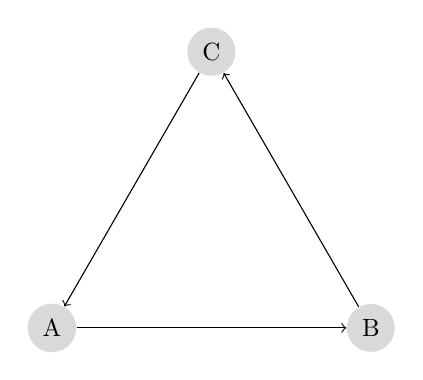
\begin{tikzpicture}[scale=.9, transform shape]
\tikzstyle{every node} = [circle, fill=gray!30]
\node (a) at (0, 0) {A};
\node (b) at +(0: 4.5) {B};
\node (c) at +(60: 4.5) {C};
\foreach \from/\to in {a/b, b/c, c/a}
\draw [->] (\from) -- (\to);
\end{tikzpicture}
\end{center}\end{frame}

\begin{frame}{Questions}\begin{center}
\Huge Questions?
\end{center}\end{frame}



\end{document}

